In autonomous systems, a fundamental task is tracking reference commands. Usually a high-level controller provides linear and angular speed references, which the robot must follow while maintaining stability and preventing falls. Our final goal will be to track reference speeds generated by a user moving a joystick, while maintaining a desired height and avoid falling.

To achieve this, the robot will have to learn a control policy that maps observations to actions. The observations will include the robot's internal states and external inputs (i.e. user commands), while the actions will be the motor positions that the robot needs to achieve to move accordingly.

\begin{highlightbox}
	\textbf{Control Policy}: The control policy maps observations to control actions. It is the brain of the robot, deciding what actions to take based on the current situation.
\end{highlightbox}

This is a really complex task, as the policy has to learn how to balance the robot, move the legs in the right way, and track the reference speeds. This is why reinforcement learning is a good approach for this task, as it allows the robot to learn from its own experience and improve over time.

\begin{figure}[!h]
	\centering
	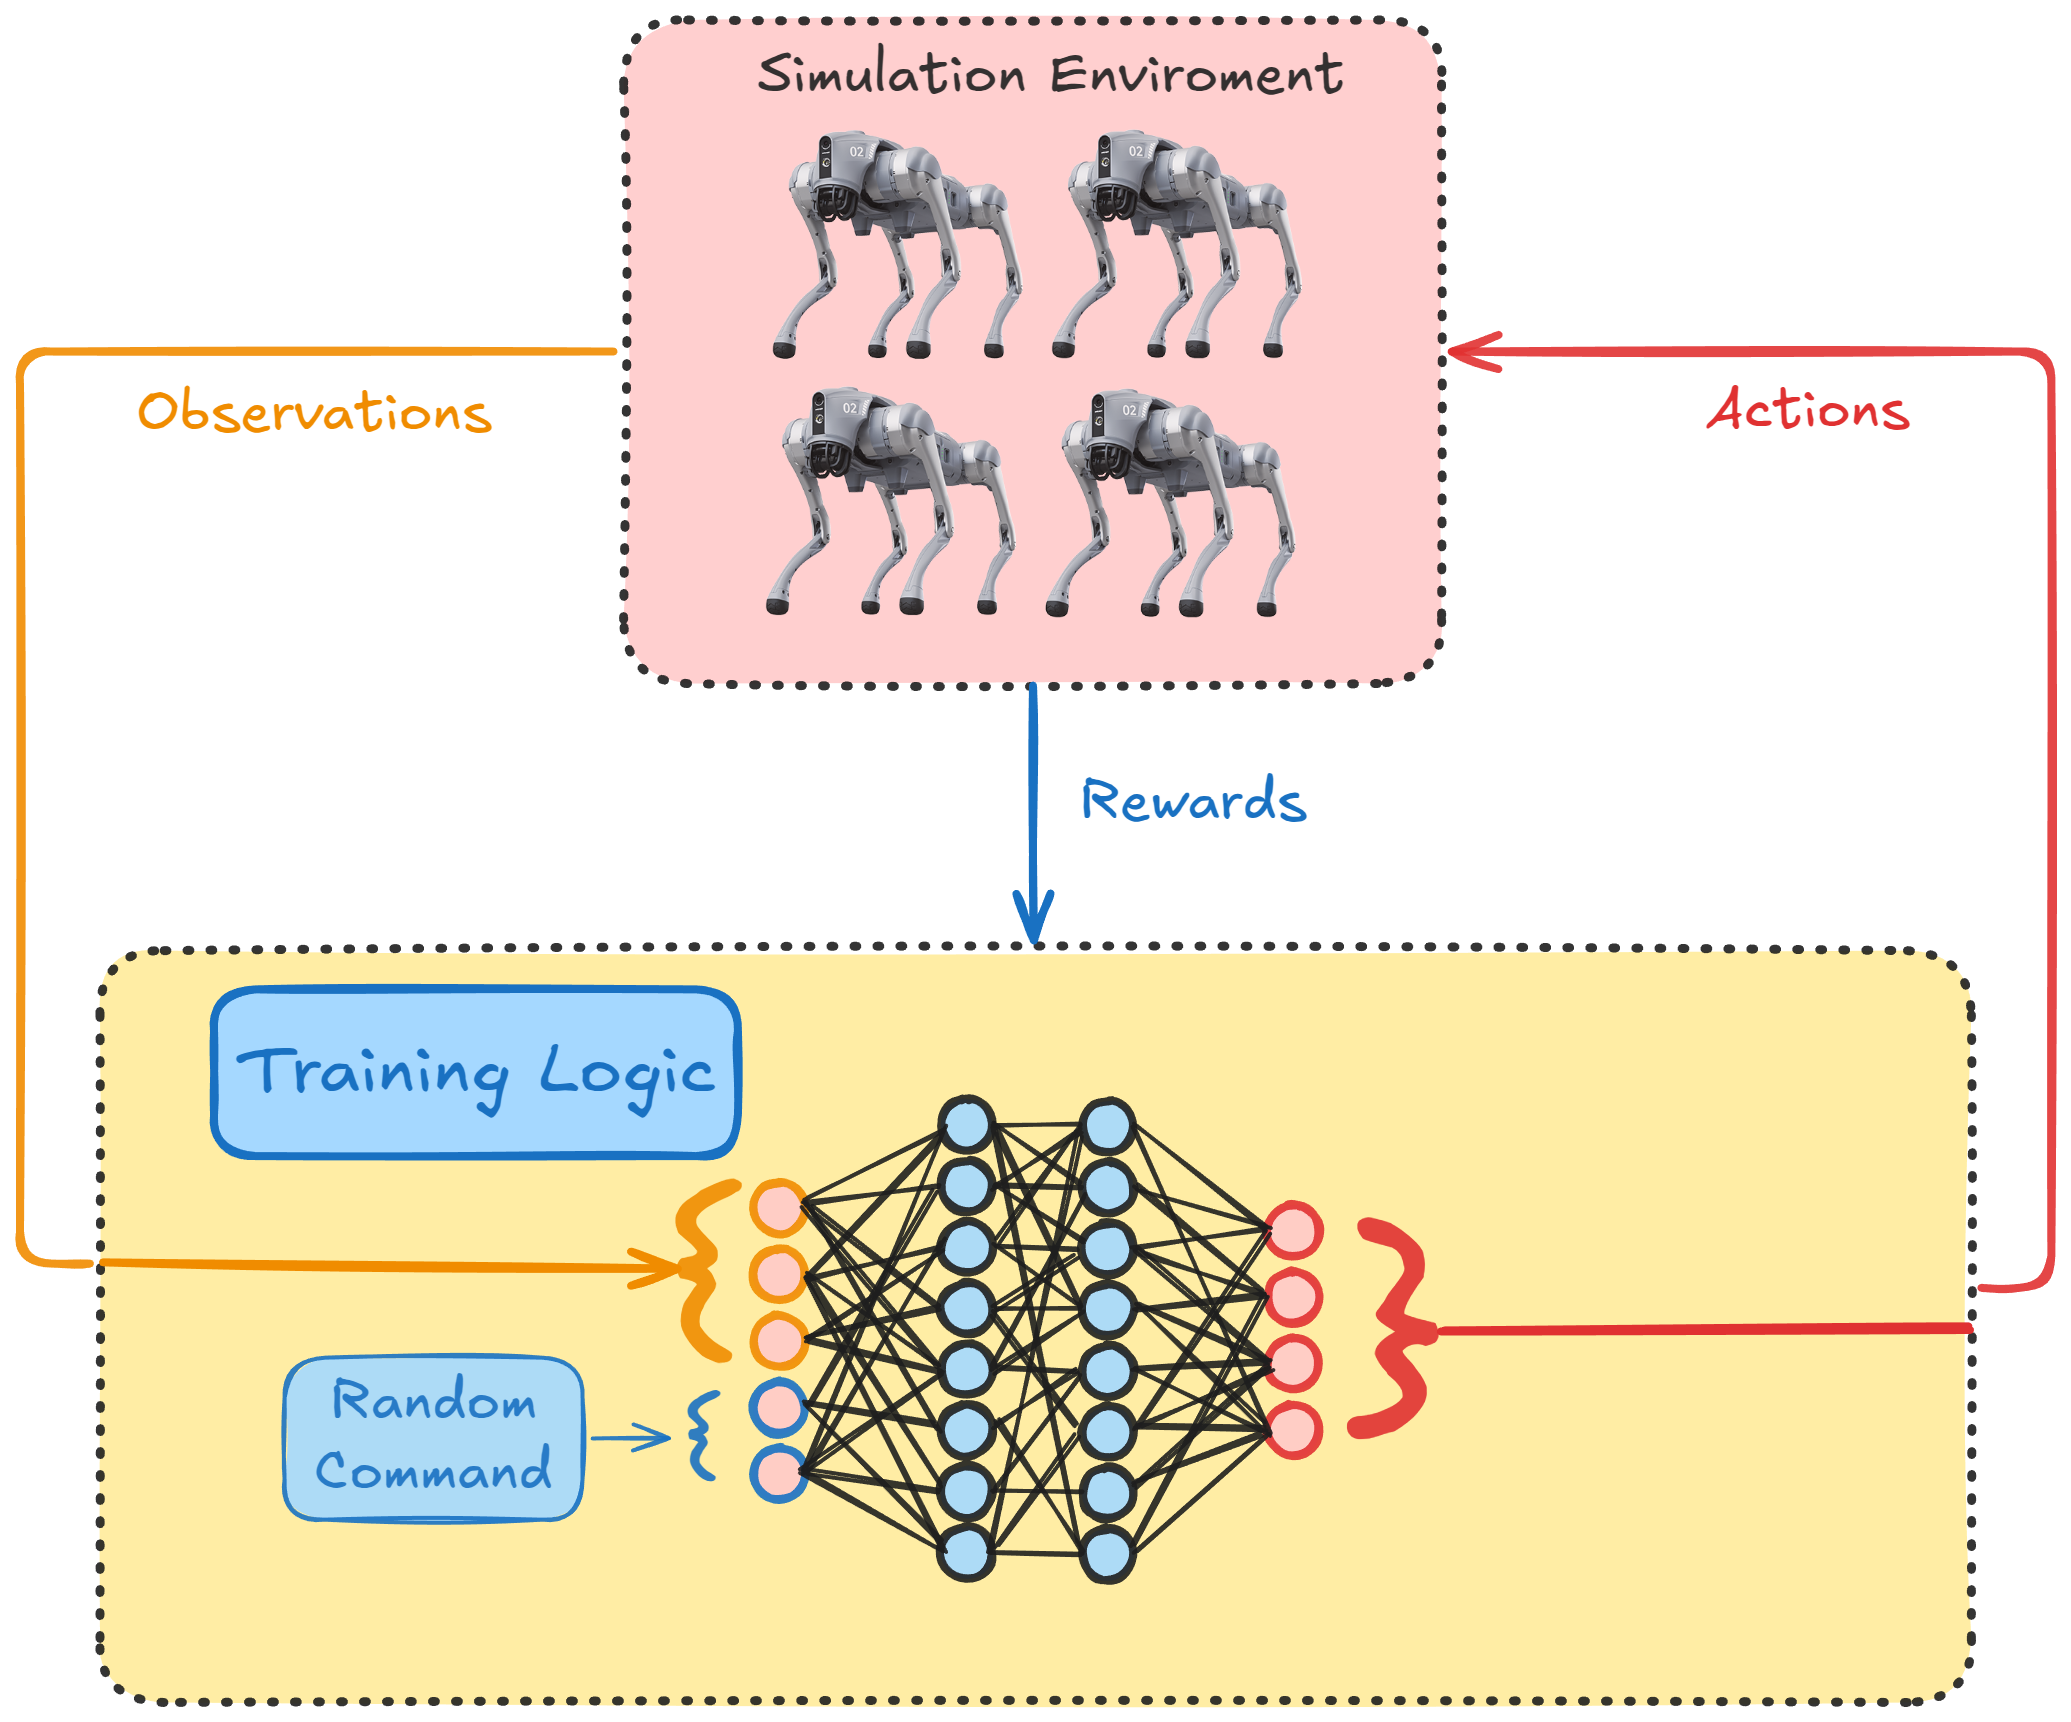
\includegraphics[width=0.5\linewidth]{fig/rl-framework}
	\caption{Reinforcement Learning Framework for Training Quadruped Robots.}
	\label{fig_sim}
\end{figure}
